
%W5100

Η χρήση του ολοκληρωμένου επιλέγεται να γίνει δια μέσω της πλακέτας WIZ811MJ της
ίδιας εταιρείας. Οι λόγοι είναι ότι επιλύει τη διασύνδεση του ολοκληρωμένου με
συνδετήρα RJ-45 (απαραίτητος για την ανταλλαγή δεδομένων μεταξύ W5100 και
δικτύου), ταλαντωτή και διάφορα άλλα ηλεκτρονικά στοιχεία. Από τους 80,
συνολικά, ακροδέκτες του W5100, το WIZ811MJ διαθέτει μόλις 40, οι οποίοι είναι
αυτοί που προορίζονται για τη διασύνδεση με μικροελεγκτή. Όλοι οι υπόλοιποι
συμμετέχουν σε εσωτερικές συνδέσεις της πλακέτας.

Ένα παράδειγμα σχετικά με το τελευταίο, το W5100 διαθέτει έναν ακροδέκτη για το
χειρισμό του ολοκληρωμένου ως Slave σε δίαυλο SPI, το \nbar{SCS}
(\textenglish{SPI Chip-Select}) \parencite[9]{wiz11:w5100}. Ωστόσο, διαθέτει και
έναν επιπρόσθετο ακροδέκτη, τον SEN (\textenglish{SPI Enable}), για την
ενεργοποίηση των υποσυστημάτων του ολοκληρωμένου για λειτουργία σε SPI
\parencite[8]{wiz11:w5100}. Το WIZ811MJ παρέχει ακροδέκτη μόνο για το \nbar{SCS}
ενώ διαθέτει κατάλληλη διάταξη ώστε η αλλαγή της τιμής του να προκαλεί το
αναμενόμενο σήμα στο SEN, αυτομάτως \parencite[7]{wiz13:811mj}.

Επιπλέον σημαντικό χαρακτηριστικό είναι ότι η πλακέτα παρέχει ακροδέκτες
συμβατούς με πρωτότυπες κάρτες (\textenglish{breadboard}) που χρησιμοποιεί η
υλοποίηση, εν αντιθέσει με το W5100 το οποίο είναι SMD
(\textenglish{Surface-Mount Device}) και απαιτεί συγκόλληση
\parencite[6,12]{wiz13:811mj}.

%Αποτελεί μία έτοιμη λύση για την προσθήκη δικτυακών δυνατοτήτων στην υλοποίηση.
%W5100 + MAG-JACK


\subsection{Επικοινωνία με μικροελεγκτή}

Το W5100 υποστηρίζει τρεις τρόπους για την επικοινωνία με το μικροελεγκτή· άμεση
ή έμμεση προσπέλαση ή, μέσω πρωτοκόλλου SPI \parencite[59]{wiz11:w5100}. Οι δύο
πρώτες μέθοδοι χρησιμοποιούν διαύλους διεύθυνσης και δεδομένων απαιτώντας πολλά
σημεία σύνδεσης με το μικροελεγκτή· για την ακρίβεια, 3 γραμμές ελέγχου
(\textenglish{Chip-Select, Read, Write}), 8 γραμμές για το δίαυλο δεδομένων,
και, 15 ή 2 γραμμές διεύθυνσης για άμεση ή έμμεση προσπέλαση, αντίστοιχα. Στην
περίπτωση του SPI απαιτούνται πολύ λιγότερες (μόλις 4) και αυτός είναι ο λόγος
που προτιμάται για τη διασύνδεση του με την MCU, δεδομένου του περιορισμένου
αριθμού ακροδεκτών της. Σαφώς, το μειονέκτημα χρήσης SPI -- ενός σειριακού
πρωτοκόλλου επικοινωνίας -- είναι ότι επιτυγχάνεται πολύ μικρότερος ρυθμός
ανταλλαγής δεδομένων από ότι στην περίπτωση των άλλων δύο, κάτι που, τελικά,
επηρεάζει το χρόνο απόκρισης στα εισερχόμενα αιτήματα. Ωστόσο, κρίνεται ότι για
τις ανάγκες της υλοποίησης, αυτός ο περιορισμός είναι αμελητέος σε σχέση με την
εξοικονόμηση ακροδεκτών που επιφέρει η χρήση SPI.

\begin{figure}
    \caption{Πλακέτα WIZ811MJ και διάταξη των ακροδεκτών του W5100.
    \label{fig:net:811mj-pins}}
    \begin{center}
    \includegraphics[width=0.9\textwidth]{network_811mj_pin-layout}
    \end{center}
    \fullcite[6]{wiz13:811mj:pins}
\end{figure}

% συνδεσμολογία
Το σχήμα \ref{fig:net:811mj-pins} παρουσιάζει την πλακέτα WIZ811MJ και, σε
μεγέθυνση, την ονομασία των ακροδεκτών της. Από τους ακροδέκτες J1, ιδιαίτερου
ενδιαφέροντος είναι οι 1 (MOSI), 2 (MISO) και 12 (3V3D) εκ των οποίων οι δύο
πρώτοι χρησιμοποιούνται για την μετάδοση των bit του \textenglish{Master} και
του ενεργού \textenglish{Slave} του διαύλου SPI, αντίστοιχα, ενώ ο τελευταίος,
για την τροφοδοσία της πλακέτας με τάση 3.3V. Οι υπόλοιποι, με εξαίρεση τον 20
(\textenglish{Not Connected}), συνδέονται με την τάση αναφοράς, δεδομένου ότι
όλοι, με εξαίρεση τον ακροδέκτη 11 (GND), χρησιμοποιούνται μόνο στην περίπτωση
άμεσης ή έμμεσης προσπέλασης.

Από τους ακροδέκτες J2, ο 1 (3V3D) χρησιμοποιείται για τροφοδοσία 3.3V ενώ οι
9, 10, 19 και 20 (GND) συνδέονται με την τάση αναφοράς. Οι 3 (SCLK) και
(\nbar{SCS}) αποτελούν μέρος του διαύλου SPI για τη μεταφορά του ρολογιού από
το \textenglish{Master} και την ενεργοποίηση του W5100 ως \textenglish{Slave}.
Σύμφωνα με το εγχειρίδιο της \textcite[8]{wiz13:811mj}, ο ακροδέκτης 2
(\nbar{RESET}) προκαλεί την αρχικοποίηση όλων των καταχωρητών του W5100 στις
προεπιλεγμένες τους τιμές και κρίνεται ότι αρκεί να συνδεθεί με το αντίστοιχο
σήμα του μικροελεγκτή ώστε η αρχικοποίηση του W5100 να πραγματοποιείται μαζί
με το μικροελεγκτή.

Οι ακροδέκτες 5 (\nbar{WR}), 6 (\nbar{RD}) και 7 (\nbar{CS}) χρησιμοποιούνται
στην περίπτωση επικοινωνίας μέσω άμεσης ή έμμεσης προσπέλασης και όχι σε SPI
\parencite[8]{wiz11:w5100}. Ωστόσο, επειδή είναι \textenglish{active low},
τίθενται σε μόνιμο λογικό 1 (3.3V), μέσω αντιστάτη, ώστε να είναι λογικά
ανενεργοί.

Μέσω του ακροδέκτη 8 (\nbar{INT}), και εφόσον έχει διευθετηθεί ακολούθως, το
W5100 αναγγέλλει την επιθυμία του για επικοινωνία με το μικροελεγκτή (για
παράδειγμα, επειδή έχουν καταφθάσει δεδομένα). Σε αντίθετη περίπτωση, ο
μικροελεγκτής είναι υποχρεωμένος να εξετάζει από μόνος του το ενδεχόμενο για
επικοινωνία. %\nref{}

Για λόγους που έχουν αναφερθεί, όλοι οι υπόλοιποι ακροδέκτες συνδέονται με την
τάση αναφοράς.

Στο σχήμα \ref{fig:network:spi_reset_int} εμφανίζεται η συνδεσμολογία του
μικροελεγκτή με τους ακροδέκτες του W5100 (δια μέσω της πλακέτα WIZ811MJ).
Αξίζει να σημειωθεί ότι, παρόλο που το W5100 λειτουργεί με τάση έως και 3.6V,
ανέχεται τάση στα σήματα εισόδου έως και 5.5V (\textenglish{5V tolerant})
\parencite[64]{wiz11:w5100}. Το χαρακτηριστικό αυτό είναι ιδιαίτερα σημαντικό
επειδή καθιστά δυνατή τη διασύνδεσή του με το μικροελεγκτή χωρίς να απαιτούνται
επιπρόσθετα ενδιάμεσα κυκλώματα για λογικό μετασχηματισμό. %\nref{}

\begin{figure}
    \caption{Διασύνδεση μικροελεγκτή και W5100.
    \label{fig:network:spi_reset_int}}
    \begin{center}
    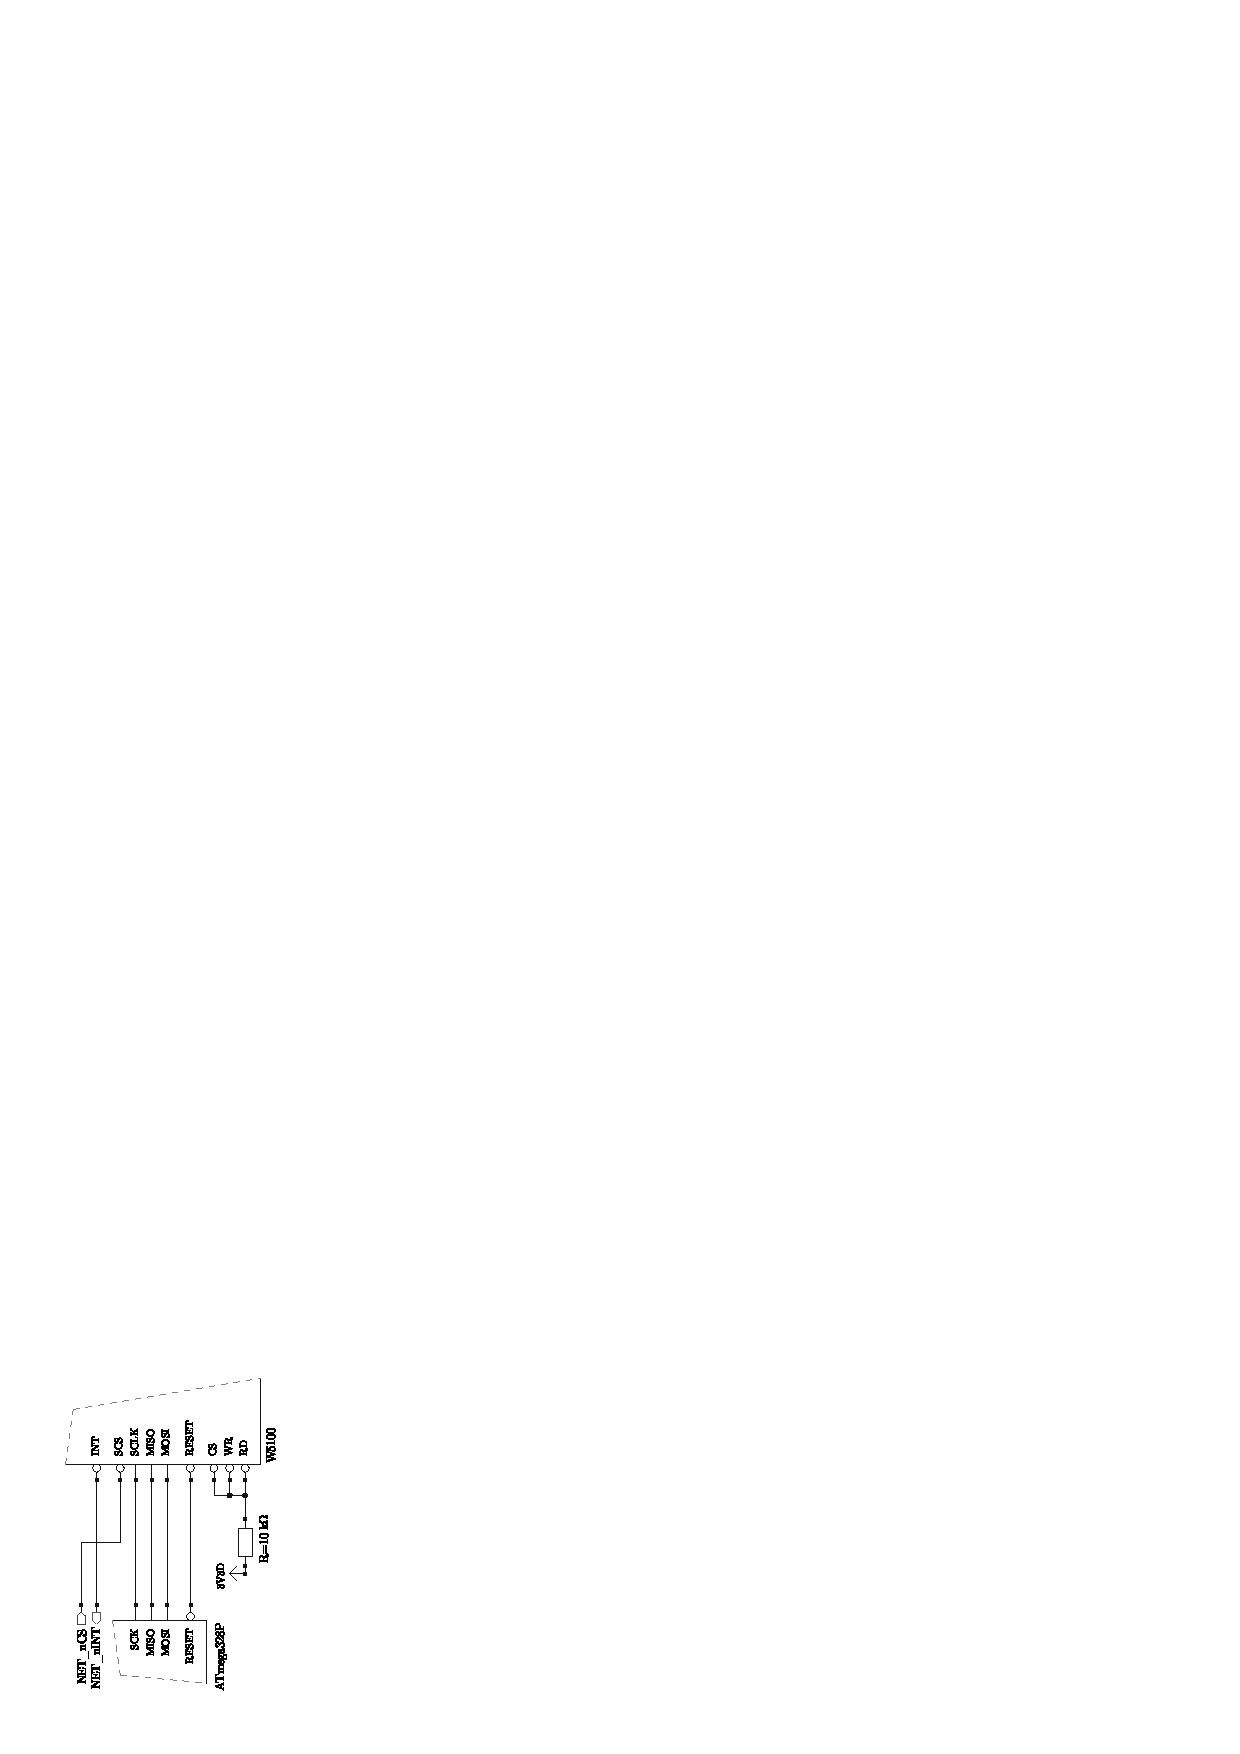
\includegraphics{network_schem_spi_reset_int}
    \end{center}
\end{figure}
